\documentclass[index]{subfiles}

\setcounter{chapter}{1}

\begin{document}
  \chapter{リプレイ}
  \label{ch:second}

この章では、実際にProgramming Partyを遊んだ内容を記録し、どういう考えで実装したのかを解説していきます。

なお、ゲームモードはソロプレイで行っており、公開するカードは基本のゲームと同じく★・★・★★・Rule Change・★★★の順になっています。

  \section{最初のゲーム}
  \label{sec:replay_first}

最初のゲームでは、とりあえず仕様通りに動くことを目指して手早く実装をしていきます。

  \subsection{基本ルール:出力}

\begin{center}
  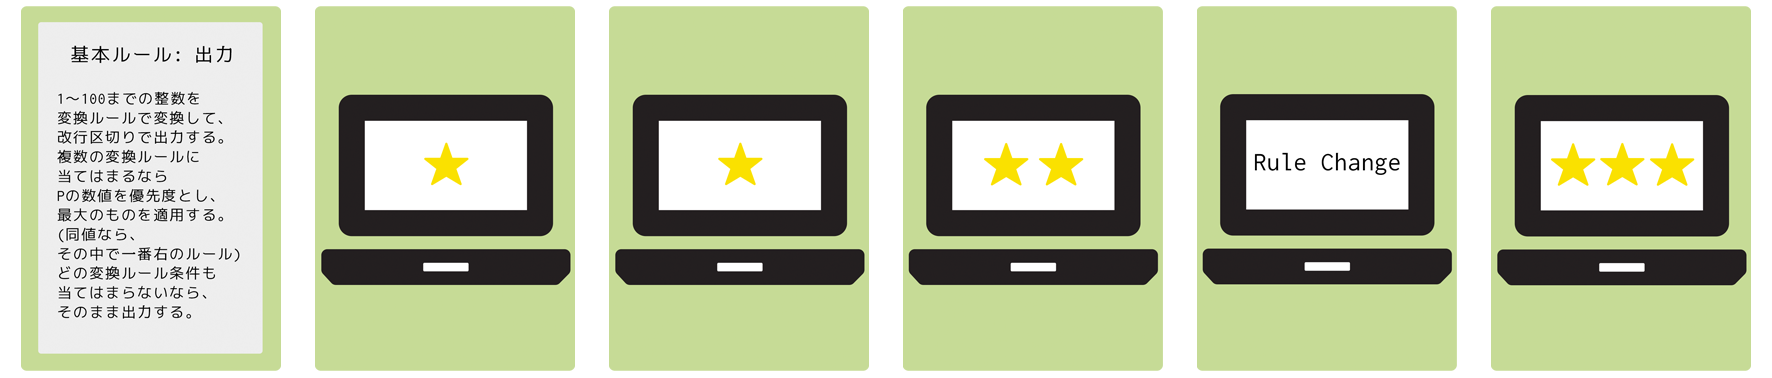
\includegraphics[height=3.2cm]{image/201_replay_first.png}
\end{center}
  
ゲームの始めは、上の画像のように「基本ルール: 出力」だけが公開された状態で、他のルールは裏向きになっています。

「基本ルール: 出力」は次に示すとおり、1から100までの整数を変換ルールに従って変換するというものです。現時点では有効な変換ルールがないので、単に1から100までの数値を順に出力するだけ、ということですね。
  
\begin{itembox}[l]{基本ルール: 出力}
1~100までの整数を変換ルールで変換して、改行区切りで出力する。

複数の変換ルールに当てはまるならPの数値を優先度とし、最大のものを適用する。(同値なら、その中で一番右のルール)

どの変換ルール条件も当てはまらないなら、そのまま出力する。
\end{itembox}

これだけなら中括弧ブロックでのワンライナーでも問題なさそうですが、この後ブロック内の処理が増えることを考慮してdoブロックにしておきましょう。

\begin{lstlisting} 
(1..100).each do |n|
  puts n
end
\end{lstlisting}

  \subsection{1枚目: ★倍数(A)}

それでは、一番左の★カードをオープンしてみましょう。表にしたカードは「倍数(A)」という仕様カードで、その下に別の★カードを組み合わせた結果、以下のようになりました。

\begin{center}
  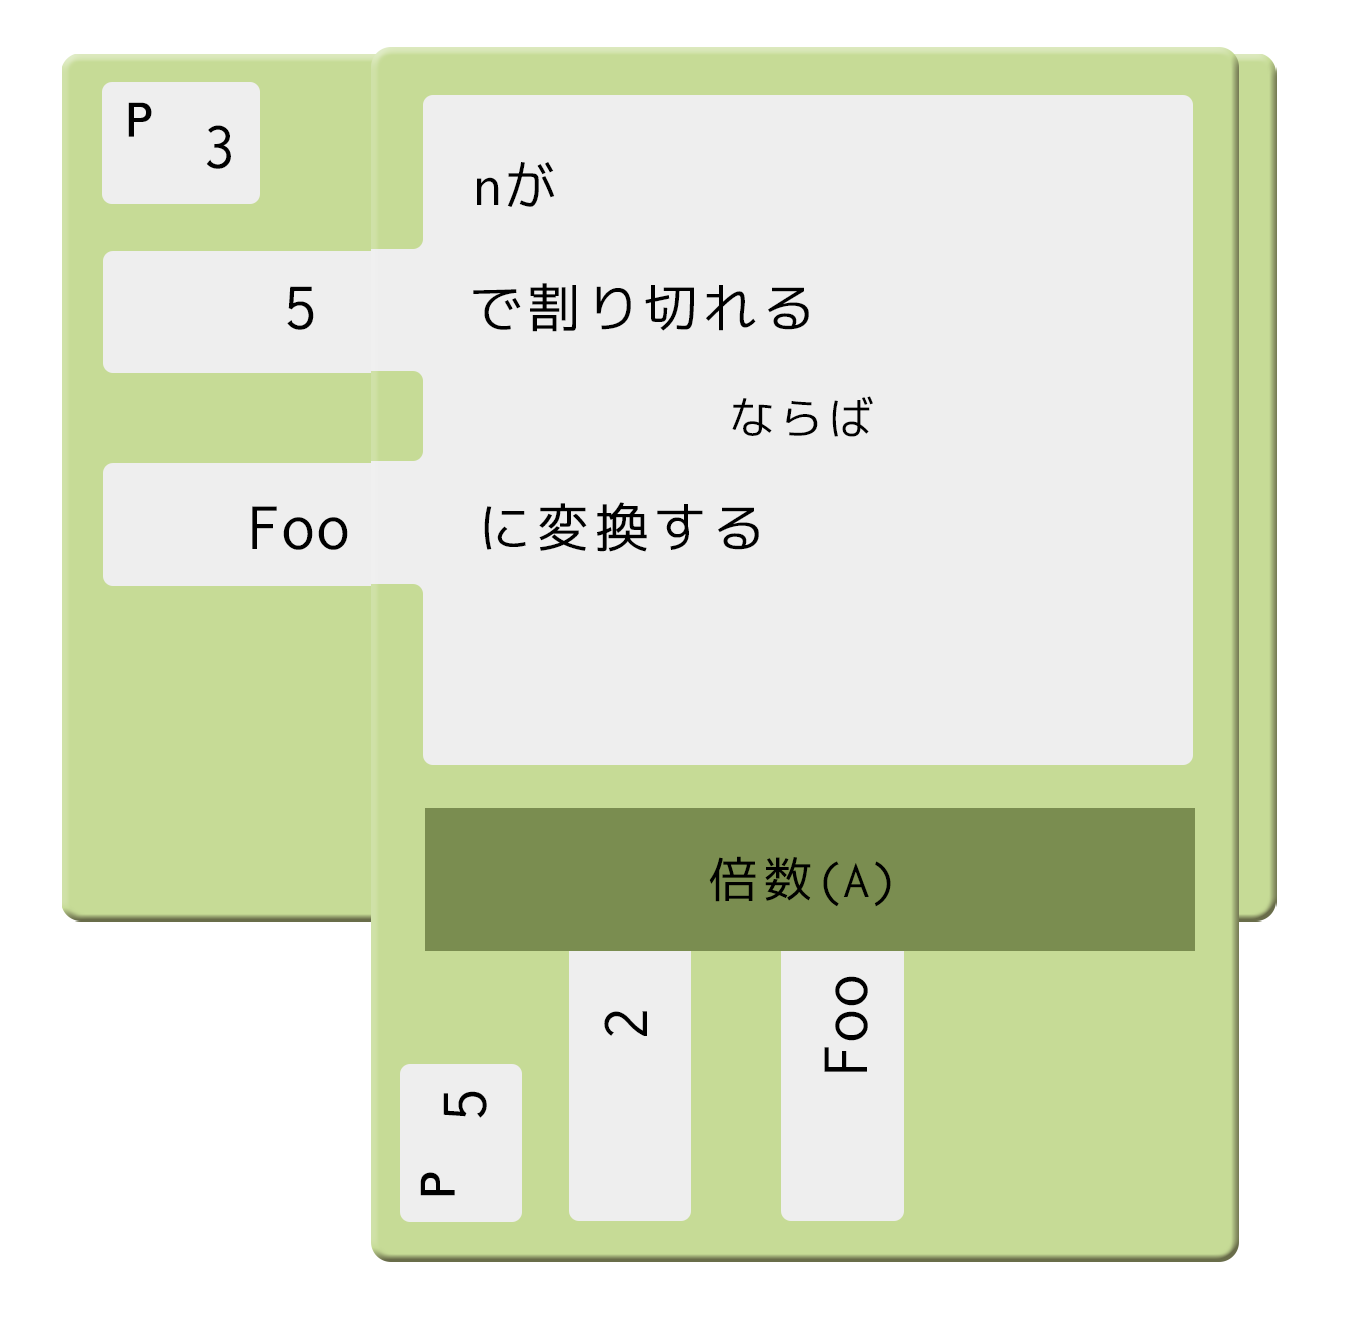
\includegraphics[height=4cm]{image/202_replay_1_1.png}
\end{center}

\begin{itembox}[l]{倍数(A)}
Pの数値: 3

nが5で割り切れるならば、Fooに変換する
\end{itembox}

まぁ、これは簡単ですね。書いてあるとおり、5で割り切れるかをif文でチェックすれば十分でしょう。

\begin{lstlisting}
(1..100).each do |n|
  if n % 5 == 0 then
    puts 'Foo'
  else
    puts n
  end
end
\end{lstlisting}

これを実行すると、 \verb+1, 2, 3, 4, Foo, 6, 7, 8, 9, Foo, 11, ...+ といった出力が得られます。きちんと5で割り切れる数のときだけFooになっており、それ以外ではそのまま出力されていますね。

  \subsection{2枚目: ★各桁の合計(B)}

次のカードは「各桁の合計(B)」でした。指標カードも組み合わせると以下のようになります。

\begin{center}
  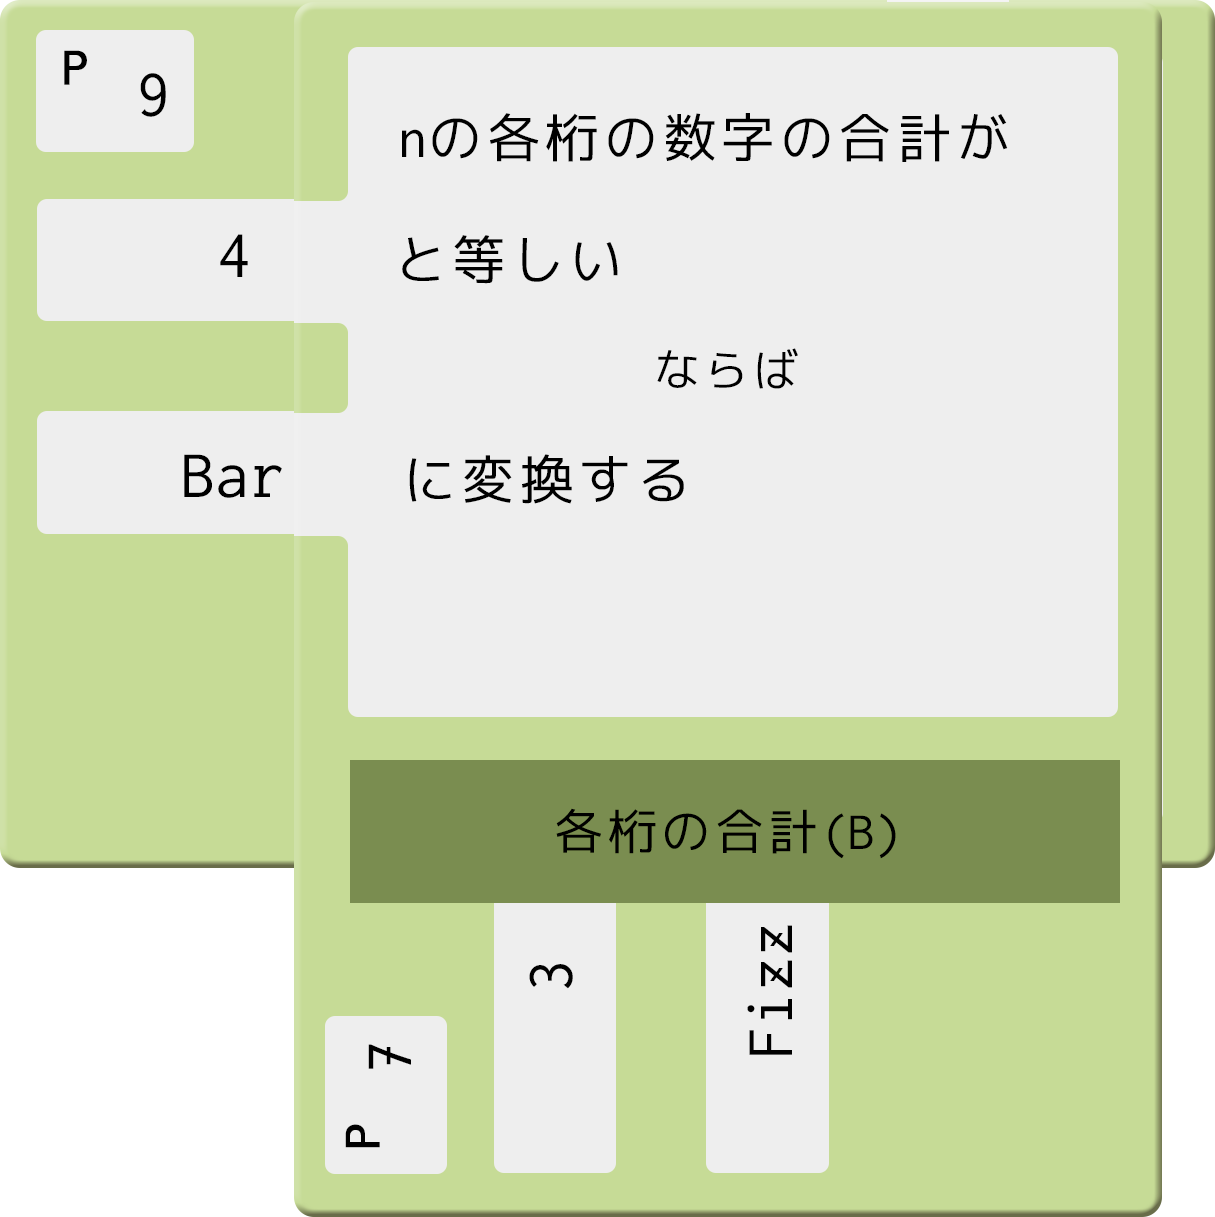
\includegraphics[height=4cm]{image/202_replay_1_2.png}
\end{center}

\begin{itembox}[l]{倍数(A)}
Pの数値: 9

nの各桁の数字の合計が4と等しいならば、Barに変換する
\end{itembox}

「各桁の数字の合計」を取るのは少々面倒そうです。例えば62だった場合は6+2=8と計算するわけですね。

基本ルールによって変換する数値が1から100に限られているため「1の位を取る式」と「10の位を取る式」と「100の位を取る式」を組み合わせれば実現はできそうです。しかしながら、もっと手軽にできる方法はないでしょうか?

Rubyでは、\verb+split+メソッドを使って1つの文字列を複数に分割することができます。この際、\verb+split(//)+のように空の正規表現を渡すことで、1文字ずつに分割することができます。

これを利用すれば、\verb+62+という数値を\verb+['6', '2']+という文字列の配列にすることができそうです。あとはそれぞれを数値にして足し合わせれば、「各桁の数字の合計」を綺麗に取ることができますね。

この考えを元に実装したのが以下のコードです。

\begin{lstlisting}
(1..100).each do |n|
  if n.to_s.split(//).map(&:to_i).sum == 4 then
    puts 'Bar'
  elsif n % 5 == 0 then
    puts 'Foo'
  else
    puts n
  end
end
\end{lstlisting}

まさに先ほど説明した通りの流れになっていますね。本来は責務をもう少し分割するべきでしょうが、今回は手っ取り早く動かす方針なのでこのままにしておきましょう。

なお、基本ルールに「複数の変換ルールに当てはまるならPの数値を優先度とし、最大のものを適用する」とあるため、Pの数値が9である「各桁の合計」の判定を先に持ってきています。

  \subsection{3枚目: ★★平方数}

次は★★のカードになるので、少し難易度が上がる……はずです。

\begin{center}
  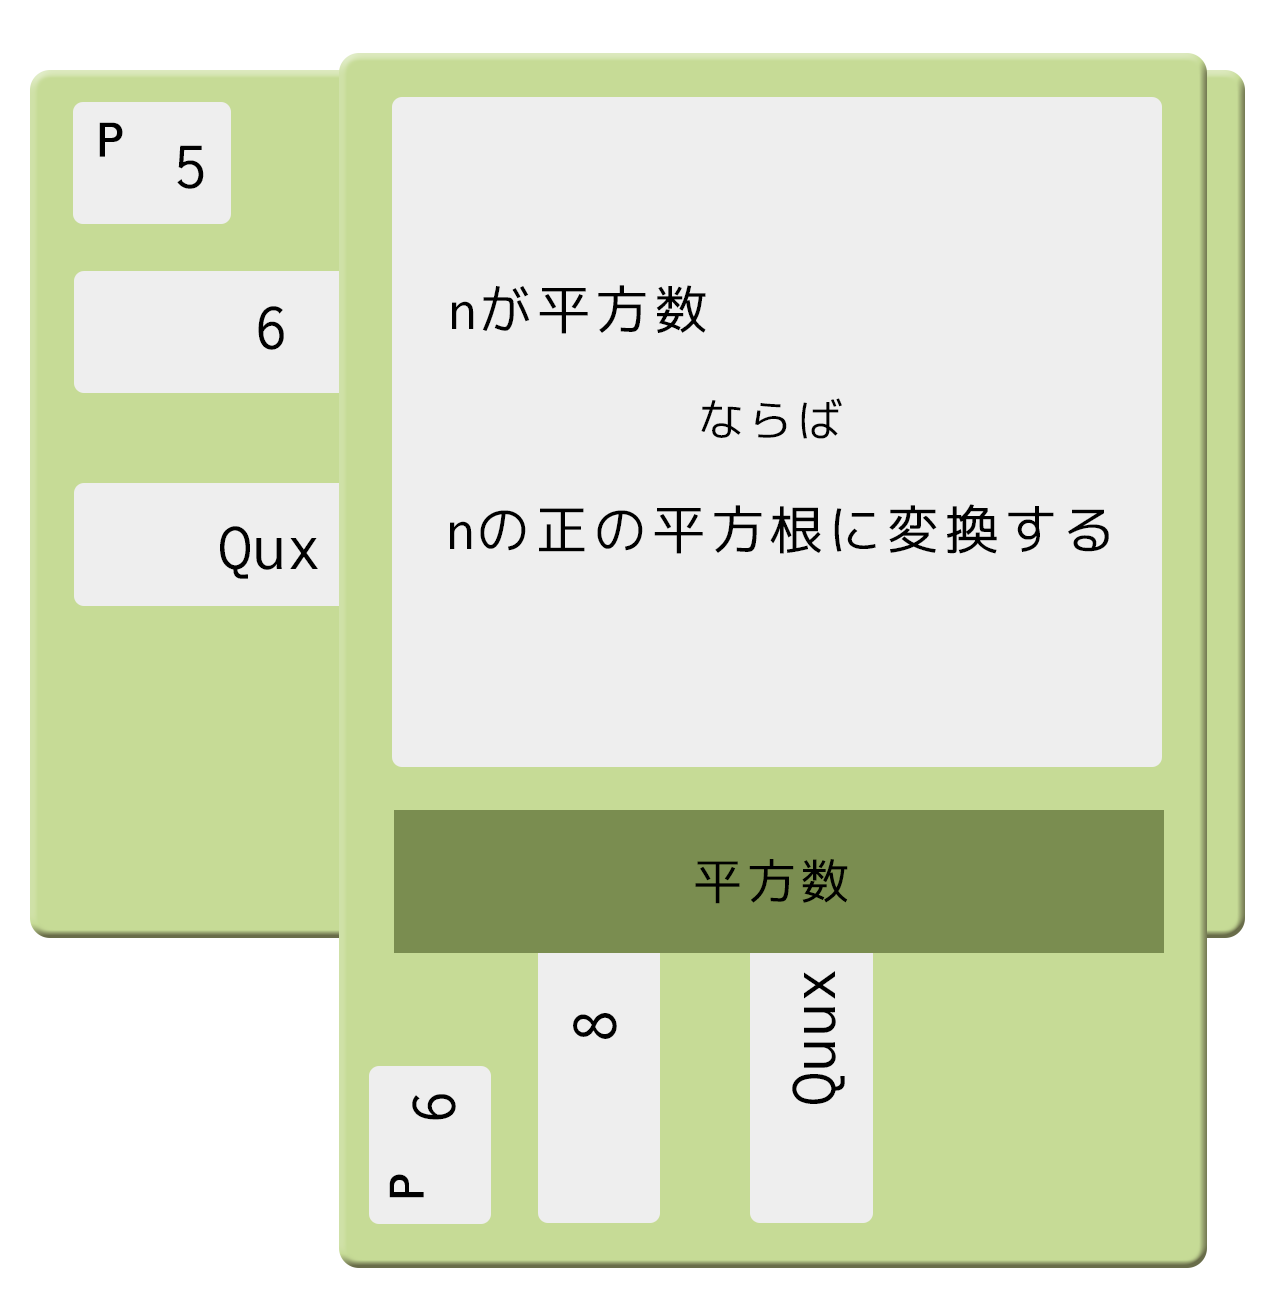
\includegraphics[height=4cm]{image/203_replay_1_3.png}
\end{center}

\begin{itembox}[l]{平方根}
Pの数値: 5

nが平方数ならば、nの正の平方根に変換する
\end{itembox}

平方数かの判定は、1から順に平方数のリストを作っておく方法と、平方根を取って整数になっているかをチェックする方法の2つがぱっと思いつきました。今回は後者で実装していきましょう。

整数判定は、\verb+to_i+した結果が自身と等しいかで行うことにします。これをワンライナーでやるのはさすがに読みにくくなりそうなので、\verb+square?+メソッドを切り出しておきましょう。

\begin{lstlisting}
def square?(n)
  m = Math.sqrt(n)
  m == m.to_i
end
\end{lstlisting}

判定メソッドさえできれば、後は簡単ですね。今回の変換ルールは「Pの数値」が他2つの中間なので、判定も間に挟み込んでいきましょう。

\begin{lstlisting}
(1..100).each do |n|
  if n.to_s.split(//).map(&:to_i).sum == 4 then
    puts 'Bar'
  elsif square?(n)
    puts Math.sqrt(n).to_i
  elsif n % 5 == 0 then
  # ...
\end{lstlisting}

  \subsection{4枚目: 左ローテーション}

ここまで★・★・★★と3枚の仕様カードに従って実装してきましたが、ここで初めてRule Changeカードをめくることになります。割と簡単な変換ルールが続きましたが、Rule Changeで難易度が化けるかどうか……?

\begin{center}
  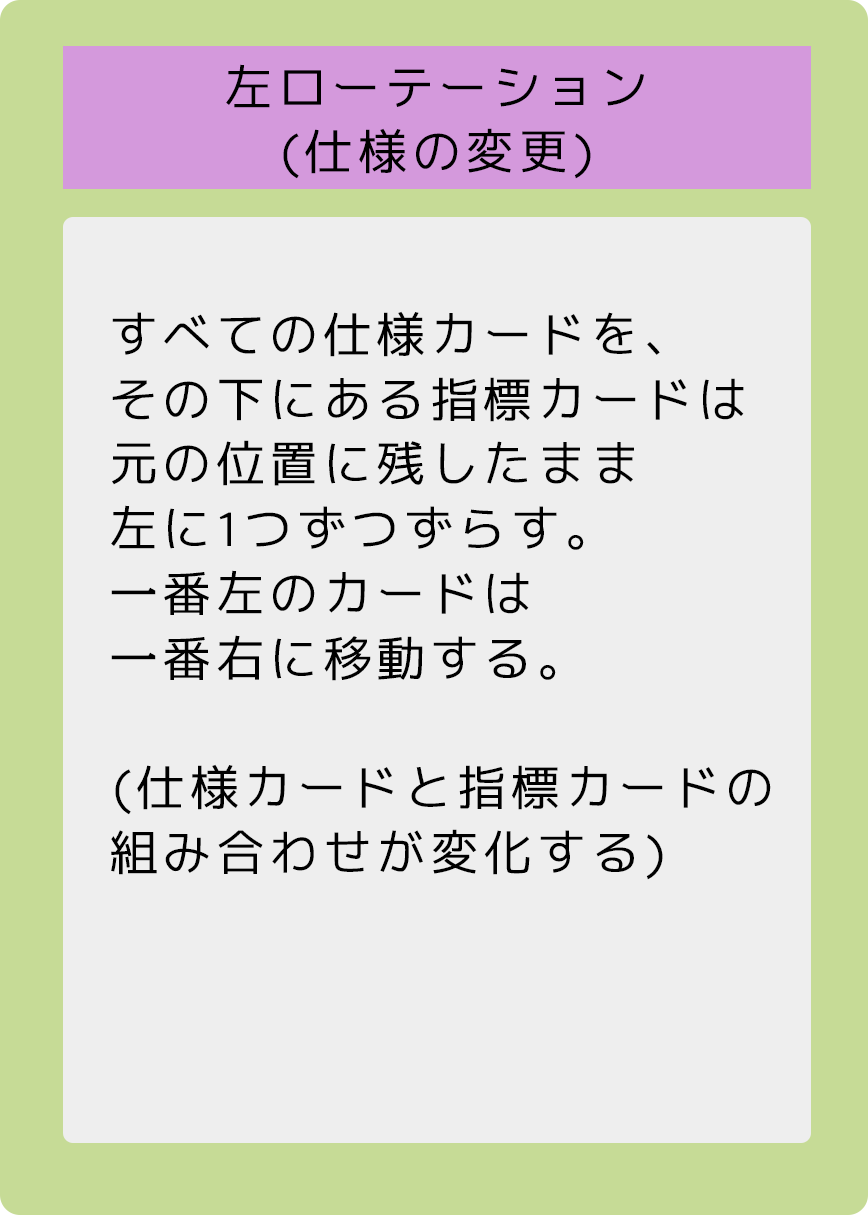
\includegraphics[height=4cm]{image/204_replay_1_4.png}
\end{center}

\begin{itembox}[l]{左ローテーション}
すべての仕様カードを、 その下にある指標カードは元の位置に残したまま 左に1つずつずらす。

一番左のカードは一番右に移動する。 (仕様カードと指標カードの組み合わせが変化する)
\end{itembox}

仕様カードの配置変更を行う「左ローテーション」カードでした。これはカードに書いてあるとおり、指標カードを残したまま仕様カードをひとつずつ左にずらし、変換ルールを全て別のものにしてしまうものです。

ここまでめくってきた仕様カードは以下のような状態になっています。

\begin{center}
  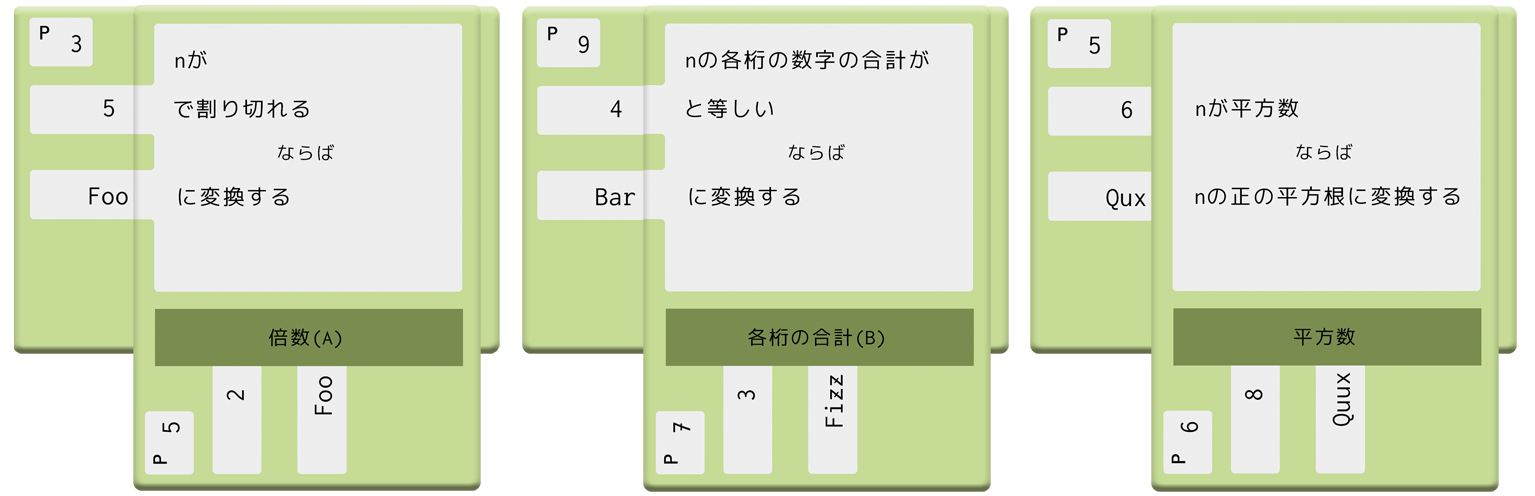
\includegraphics[height=4cm]{image/205_replay_1_5.png}
\end{center}

これを、「各桁の合計(B)」と「平方根」のカードはひとつずつ左にずらし、押し出された「倍数(A)」はもともと「平方根」があった一番右に移動します。こうしてカードを動かした結果が以下です。

\begin{center}
  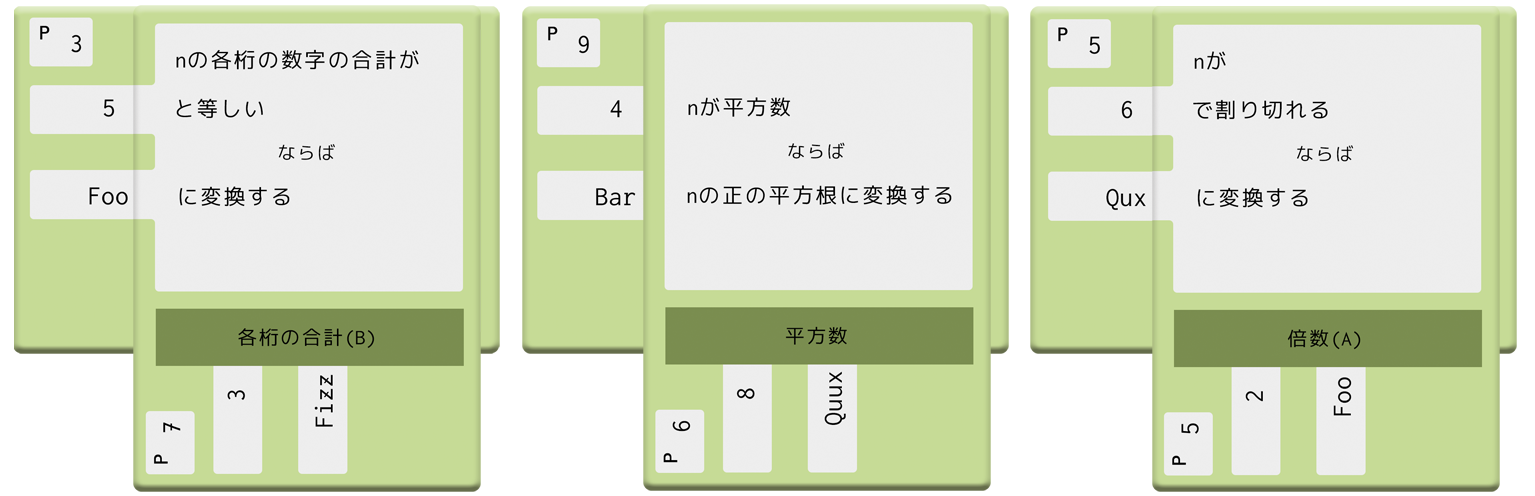
\includegraphics[height=4cm]{image/206_replay_1_6.png}
\end{center}

「各桁の合計(B)」は指標カードが変わり「nの各桁の数字の合計が5と等しいならば、Fooに変換する」という変換ルールになります。他の仕様カードも同じように変わっているため、新たな変換ルールは以下のようになります。

\begin{itembox}[l]{ローテーション後の変換ルール}
{\sf 各桁の合計(B)}

\hspace{1em}Pの数値: 3

\hspace{1em}nの各桁の数字の合計が5と等しいならば、Fooに変換する

{\sf 平方数}

\hspace{1em}Pの数値: 9

\hspace{1em}nが平方数ならば、nの正の平方根に変換する

{\sf 倍数(A)}

\hspace{1em}Pの数値: 5

\hspace{1em}nが6で割り切れるならば、Quxに変換する
\end{itembox}

そこまで大きくは変わっていないですね。とはいえ判定に使う数値だけではなくPの数値も変わっているので、判定の順序も入れ替える必要があることには注意が必要そうです。

もともとは「各桁の合計(B)」「平方数」「倍数(A)」という優先順でしたが、新しいルールでは「平方数」「倍数(A)」「各桁の合計(B)」の順になります。この順序の入れ替えと、判定に使う数値や出力文字列の変更を合わせて、コードのdiffは以下のようになりました。

\begin{lstlisting}
 (1..100).each do |n|
-  if n.to_s.split(//).map(&:to_i).sum == 4 then
-    puts 'Bar'
-  elsif square?(n)
+  if square?(n)
     puts Math.sqrt(n).to_i
-  elsif n % 5 == 0 then
+  elsif n % 6 == 0 then
+    puts 'Qux'
+  elsif n.to_s.split(//).map(&:to_i).sum == 5 then
     puts 'Foo'
   else
     puts n
\end{lstlisting}

  \subsection{5枚目: ★★★三次方程式}

最後はもっとも難易度の高い★★★の仕様カードです。さて、何が出てくるか。

\begin{center}
  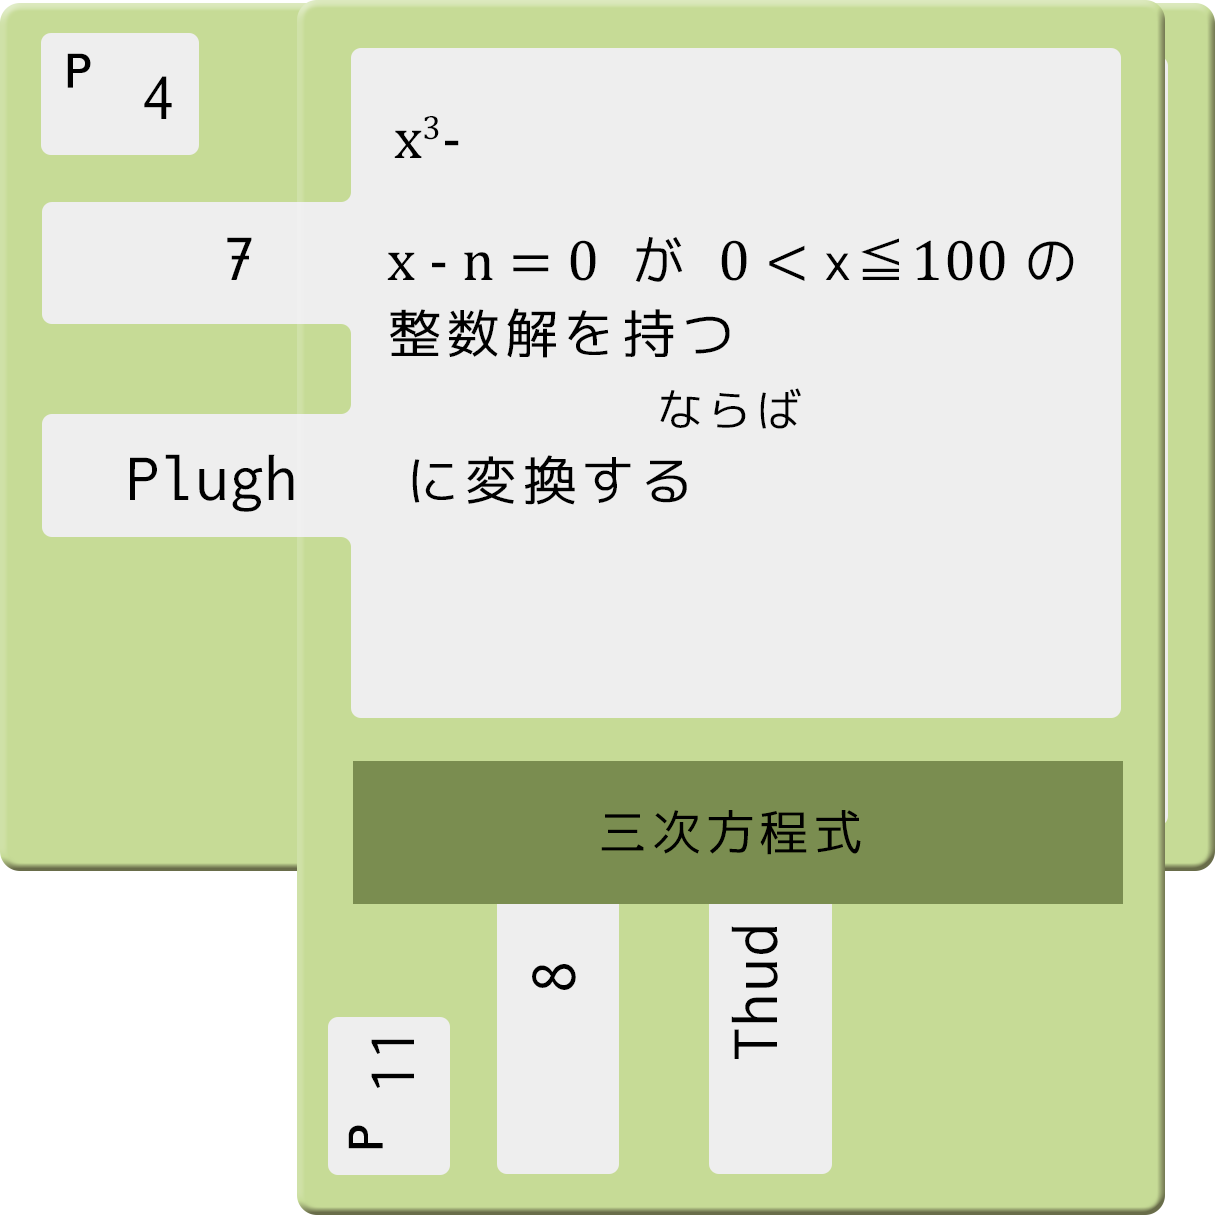
\includegraphics[height=4cm]{image/207_replay_1_7.png}
\end{center}

\begin{itembox}[l]{三次方程式}
Pの数値: 4

$x^3-7x - n = 0$ が $0 < x ≦ 100$の整数解を持つならば、Plughに変換する
\end{itembox}

三次方程式の解を求める問題です。これは指標カードによって1次の係数が変わり、今回は7になっています。

三次方程式は普通に解くと相当大変ですが、この仕様カードでは解の範囲が限られているためループで回してしまう力技で解くことができますね。

\begin{lstlisting}
def solvable?(n)
  (1..100).any? do |x|
    x ** 3 - 7 * x - n == 0
  end
end
\end{lstlisting}

\verb+solvable?(n)+は $x^3 - 7x - n = 0$ について、指定された解の範囲である1から100までの整数の中に式を満たす$x$があるかを検査しています。

あとはPの数値に気をつけて適切な場所に条件判定を入れれば良さそうですね。

これでこのゲームのプログラムは完成になるので、完全なソースコードを以下に掲載しておきます。

\begin{lstlisting}
def square?(n)
  m = Math.sqrt(n)
  m == m.to_i
end

def solvable?(n)
  (1..100).any? do |x|
    x ** 3 - 7 * x - n == 0
  end
end

(1..100).each do |n|
  if square?(n)
    puts Math.sqrt(n).to_i
  elsif n % 6 == 0 then
    puts 'Qux'
  elsif solvable?(n) then
    puts 'Plugh'
  elsif n.to_s.split(//).map(&:to_i).sum == 5 then
    puts 'Foo'
  else
    puts n
  end
end
\end{lstlisting}

構造化を意識せずさっくりと実装することを重視しましたが、引いた仕様が比較的簡単だったこともあり短くシンプルな実装になったのではないでしょうか。

  \section{2度目のゲーム}
  \label{sec:replay_second}

さて、最初のゲームではややあっさりした仕様ばかり引いてしまった感がありますので、再度プレイしてみましょう。今回はプログラムをある程度構造化し、処理に意味のある名前をつけることを意識して実装していきます。

  \subsection{1枚目: ★各桁の合計}

基本ルールは先と同じく「基本ルール: 出力」とし、1から100までを出力するプログラムも同じ実装からスタートしましょう。

最初の★1カードは以下になりました。

\begin{center}
  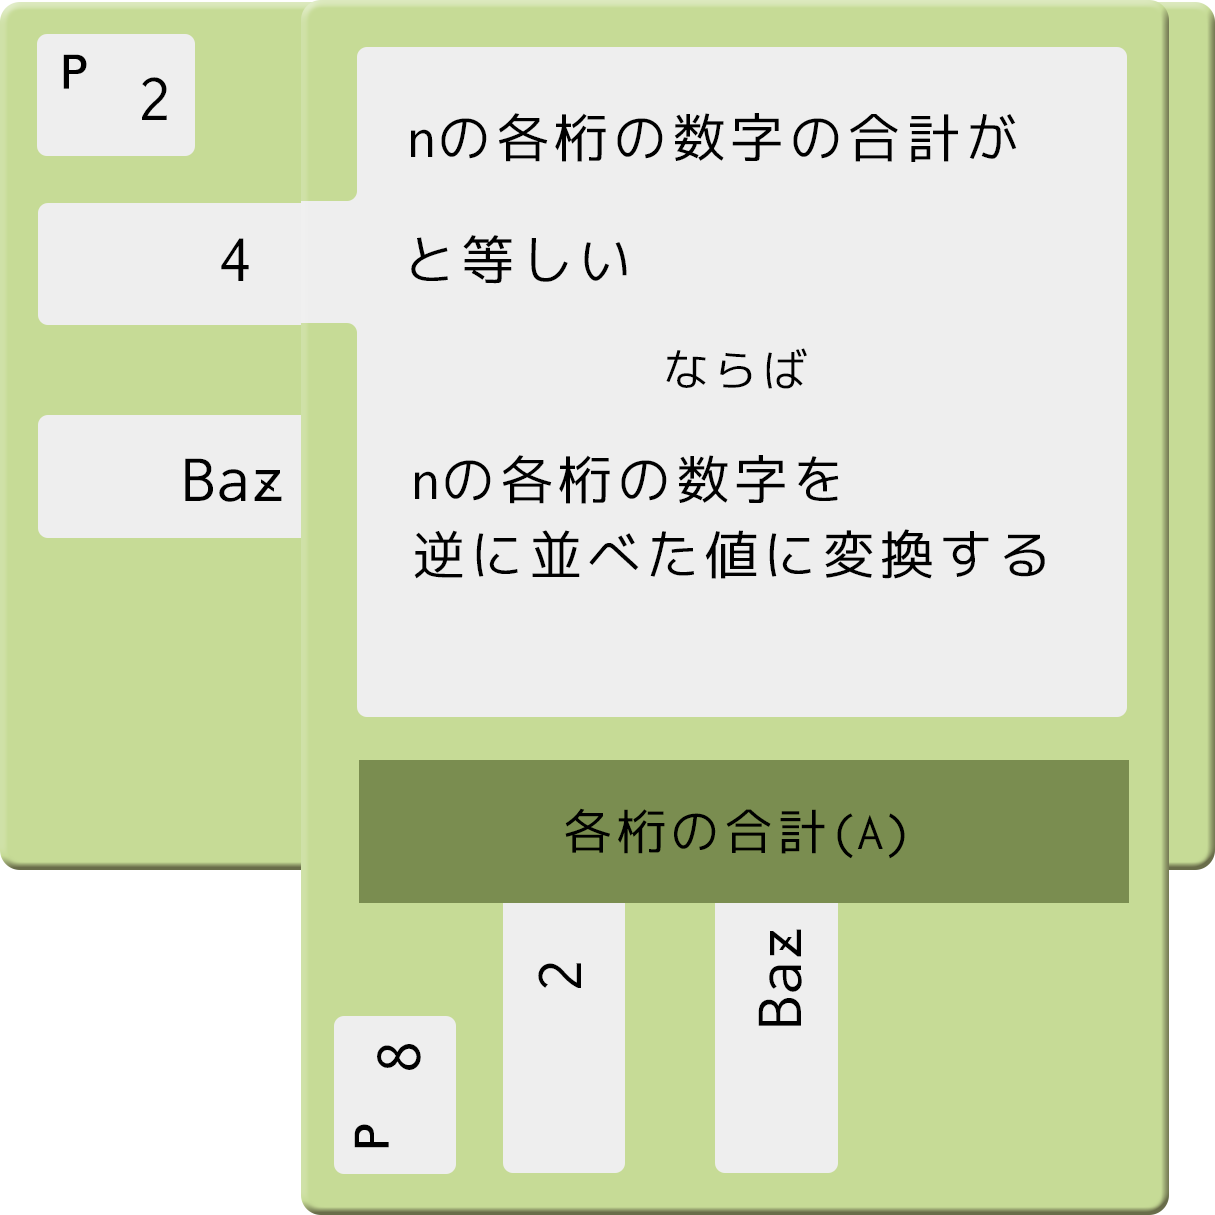
\includegraphics[height=4cm]{image/211_replay_2_1.png}
\end{center}

\begin{itembox}[l]{各桁の合計(A)}
Pの数値: 2

nの各桁の数字の合計が4と等しいならば、nの各桁の数字を逆に並べた値に変換する
\end{itembox}

各桁の数字の合計は、最初のゲームでも求める処理がありましたね。ただし今回は、条件を満たした場合に「各桁の数字を逆に並べた値に変換する」という捻りが加わっています。

今回は「各桁の数字」という概念が繰り返し出てくることに着目し、これをクラス化して表すことにしましょう。

\begin{lstlisting}
class Digits
  def initialize(n)
    @digits = [n / 100, n / 10 % 10, n % 10]
      .drop_while { |d| d == 0}
  end

  def sum
    @digits.sum
  end

  def reverse
    @digits.reverse.join.to_i
  end
end
\end{lstlisting}

\verb+Digits+クラスは数値を受け取り、各桁の数字の並びを保持します。なお、入力となる数値は1から100に絞られているため、\verb+initialize+での各桁を取る処理は上限3桁を決め打ちしています。

\verb+sum+は各桁の合計を、\verb+reverse+は各桁を逆に並べた数値を、それぞれ返すメソッドです。なお1桁や2桁の数を\verb+reverse+で逆に並べた際、上位の桁に0が入っているとおかしなことになってしまいます。このため、\verb+initialize+の時点で不要な0を\verb+drop_while+で取り除くようにしています。

\verb+Digits+クラスを使えば、変換ルールは簡単に書くことができますね。とはいえ、このあと変換ルールが増えていくことを踏まえて、変換自体も\verb+Converter+という1つのクラスで表して置くことにしましょう。

\begin{lstlisting}
class Converter
  def initialize(n)
    @n = n
  end

  def digit_sum_rule
    d = Digits.new(@n)
    d.reverse if d.sum == 4
  end

  def convert
    digit_sum_rule || @n
  end
end
\end{lstlisting}

「各桁の合計(B)」のルールは\verb+digit_sum_rule+メソッドに切り出されています。これを見ると、「各桁の合計が4なら、各桁を逆順に並べた数を返す」ことがわかりやすく書かれていますね。

\verb+Converter#convert+が全ての変換ルールを適用するものです。ここで、\verb+digit_sum_rule+は変換条件を満たしていない場合\verb+nil+を返していることに注意してください。この場合は\verb+@n+を返すようにすることで、\verb+if+を使わずに変換処理の優先順を表しています。

なお、\verb+Converter+は初期化時にnを受け取るようにしています。\verb+convert+がnを受け取るインターフェイスとどちらにするか迷いましたが、各変換ルールでnを参照することを考えると、これを都度引き回すよりはインスタンスに保持できるほうがわかりやすいだろうと判断しています。

さて、下準備が長くなりましたが、\verb+Converter+を使う本体は以下のようになります。

\begin{lstlisting}
 (1..100).each do |n|
-  puts n
+  puts Converter.new(n).convert
 end
\end{lstlisting}

とてもシンプルに実装できました。この部分については、今後書き換える必要はなさそうですね。

余談ですが、このように変換処理の責務を別クラスに切り出した場合、変換処理を行う関数を実装する「基本ルール: 関数」と大差ないプログラムになります。このため基本ルールのどちらを選ぶかはゲーム性にほとんど影響しないので、使う言語の特性や参加者の好みで選んでしまって良いでしょう。

  \subsection{2枚目: ★いずれかの桁}

きちんとクラスを切り出しているのもありますが、初手から最初のゲームより難しい仕様を引いた気がします。次は何が来るかな……?

\begin{center}
  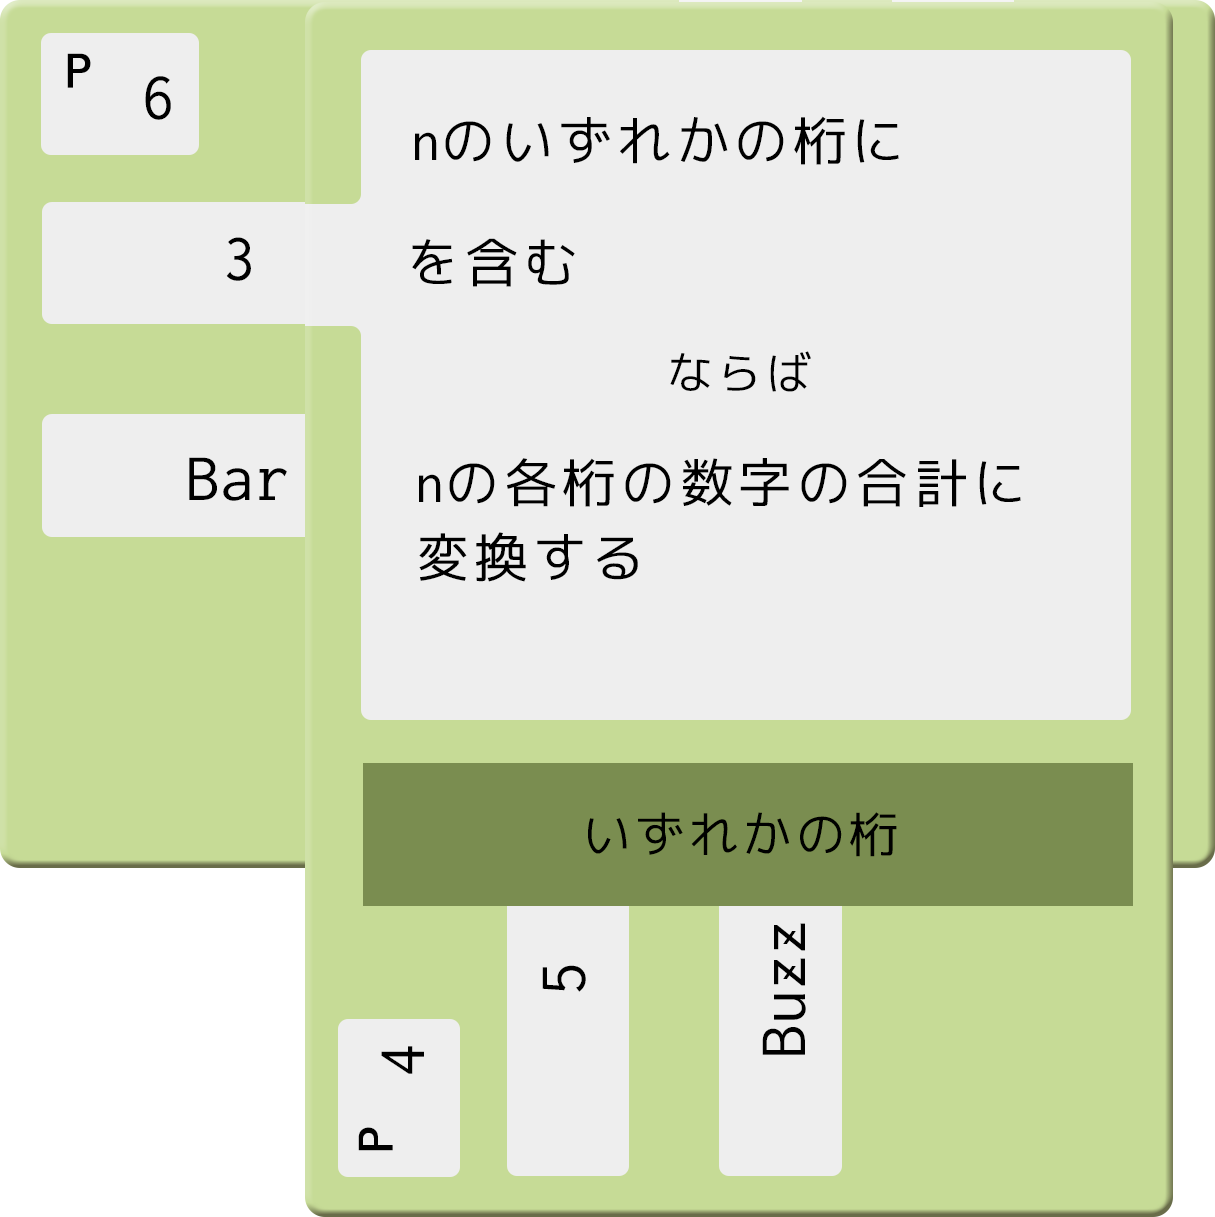
\includegraphics[height=4cm]{image/212_replay_2_2.png}
\end{center}

\begin{itembox}[l]{いずれかの桁}
Pの数値: 6

nのいずれかの桁に3を含むならば、nの各桁の数字の合計に変換する
\end{itembox}

都合よく\verb+Digits+を活かせそうなカードが来ました。ちなみに、同じ仕様になってしまわないよう最初のゲームで使ったカードは取り除いていますが、その他はランダムに引いています。

さて、「いずれかの桁にある数字を含むか」の判定は、明らかに\verb+Digits+の責務でしょう。

\begin{lstlisting}
class Digits
  # ...

  def any?(m)
    @digits.any? { |d| d == m }
  end
end
\end{lstlisting}

\verb+Digits#sum+といい、ほとんど\verb+Array+に生えているメソッドへ委譲するだけで済むのが簡単ですね。

あとは\verb+Converter+から呼び出すだけですが、2つのルールから\verb+Digits+を使うことになったので、nだけでなく\verb+Digits+のインスタンスもインスタンス変数に持たせるようにします。

\begin{lstlisting}
class Converter
  def initialize(n)
    @n = n
    @digits = Digits.new(@n)
  end

  def digit_contain_rule
    @digits.sum if @digits.any?(3)
  end

  def digit_sum_rule
    d = @digits
    d.reverse if d.sum == 4
  end

  def convert
    digit_contain_rule || digit_sum_rule || @n
  end
end
\end{lstlisting}

これでOKです。なお今回のルールは最初のルールより「Pの数値」が大きいので、先に判定するようにしています。

  \subsection{3枚目: ★★7セグメント}

2つめは\verb+Digits+を活かしやすくて簡単でしたが、果たして次の★★仕様カードは何が来るでしょうか。

\begin{center}
  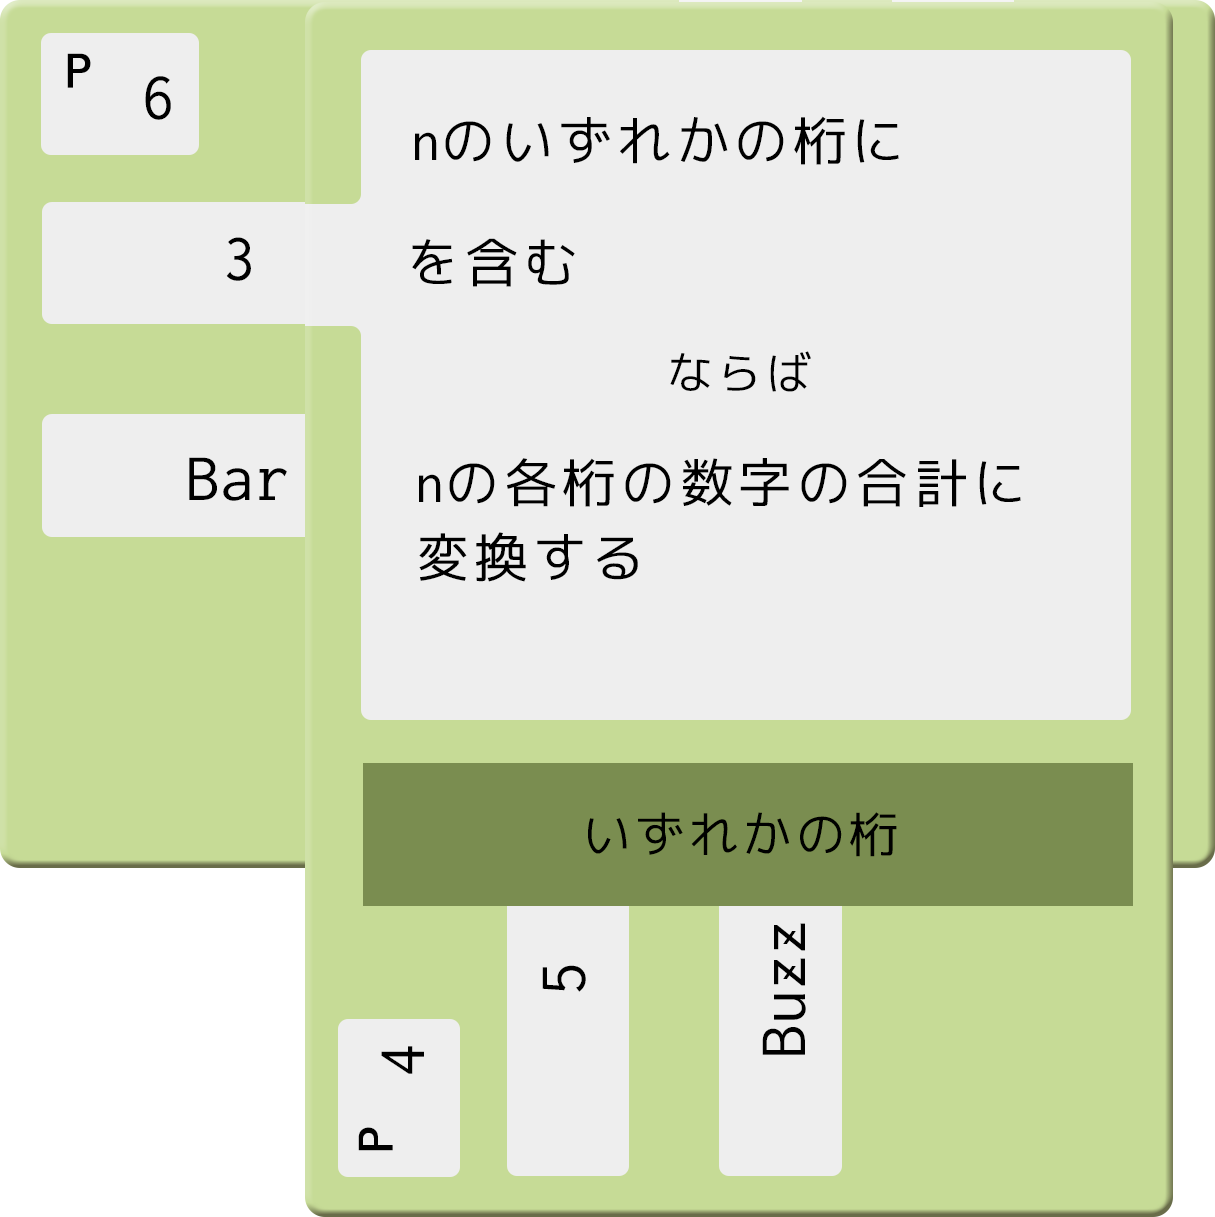
\includegraphics[height=4cm]{image/212_replay_2_2.png}
\end{center}

\begin{itembox}[l]{7セグメント}
Pの数値: 2

nの7セグメント表示を180°回転した場合に、nと等しいならば、Corgeに変換する

7セグメント表示を180°回転した場合、0, 1, 2, 5, 8はそれ自身になる。
6は9に、9は6になる。
3, 4, 7は数値にならない。
\end{itembox}

またしても結構ややこしいのを引きましたね。

7セグメント表示は電卓などで使われる表示方法で、シンプルな表示ゆえに180°回転させても数字として認識できる数字列がいくつかあったりします。今回はそういった数字のなかでも「回転させても同じ数字になる数字」を判定する変換ルールです。

これもまた\verb+Digits+を使えば割と簡単そうな雰囲気がしますね。ただ各桁に対して「7セグメント表示で180°回転させる」処理は\verb+Digits+の責務からかなり外れている感じがします。

\verb+SevenSegment+クラスを作っても良いのですが、さすがにこれ以外で7セグメントの概念を使うことはまずないでしょう。そこで今回は、\verb+Integer+に直接メソッドを生やしてしまいましょう。

\begin{lstlisting}
class Integer
  def to_flipped_7seg
    case self
    when 3, 4, 7 then nil
    when 6 then 9
    when 9 then 6
    else self
    end
  end
end
\end{lstlisting}

これで\verb+6.to_flipped_7seg+とすれば9が得られるメソッドを生やせました。Rubyのオープンクラスは多用しすぎると危険ですが、こういうちょっとした処理をするのにはとても便利ですね。

これによって、\verb+Digits+に「7セグメント表示を180°回転させた数を作るメソッド」が書きやすくなります。

\begin{lstlisting}
class Digits
  # ...
  
  def to_flipped_7seg
    flipped = @digits.map(&:to_flipped_7seg).reverse
    return if flipped.member?(nil)
    flipped.join.to_i
  end
end
\end{lstlisting}

「180°回転させる」と、各桁の数字だけではなく桁の順番も入れ替わります。このため\verb+to_flipped_7seg+しただけではなく、各桁の順序を\verb+reverse+で反転する必要があるわけですね。

また桁の中に「回転させても数字にならない」ものが含まれている可能性があるので、そういったケースを2行目で弾いています。

あとは優先度に注意しつつ\verb+Convert+に足してやりましょう。

\begin{lstlisting}
 class Converter
   # ...

+  def flipped_7seg_rule
+    'Corge' if @n == @digits.to_flipped_7seg
+  end
+  
   def convert
-    digit_contain_rule || digit_sum_rule || @n
+    digit_contain_rule || reversed_7seg_rule || digit_sum_rule || @n
   end
 end
\end{lstlisting}

  \subsection{4枚目: スワップ}

\verb+Digits+切り出したからわりと簡単に実装できてるけど、初回ゲームと比べてやけに難易度が高いような……

そんな気持ちを抱きつつ、4枚目のRule Changeをオープンしていきましょう。

\begin{center}
  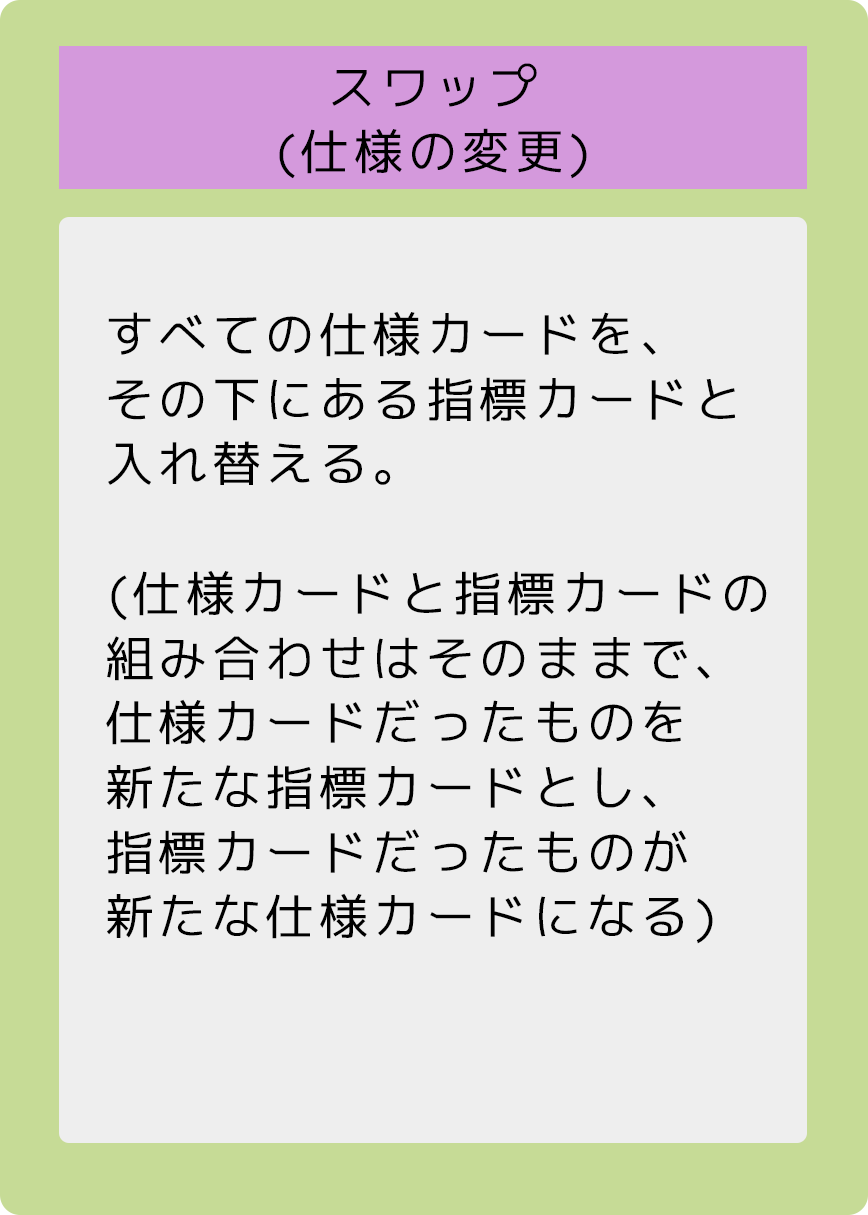
\includegraphics[height=4cm]{image/214_replay_2_4.png}
\end{center}

\begin{itembox}[l]{スワップ}
すべての仕様カードを、その下にある指標カードと入れ替える。

(仕様カードと指標カードの組み合わせはそのままで、仕様カードだったものを新たな指標カードとし、指標カードだったものが新たな仕様カードになる)
\end{itembox}

あー、スワップ引いちゃいましたか。これは結構大変そう……

このカードは「各仕様カードを、その下にある指標カードと入れ替える」効果を持ちます。どう変わるか見るのが手っ取り早いでしょうか。

\begin{center}
  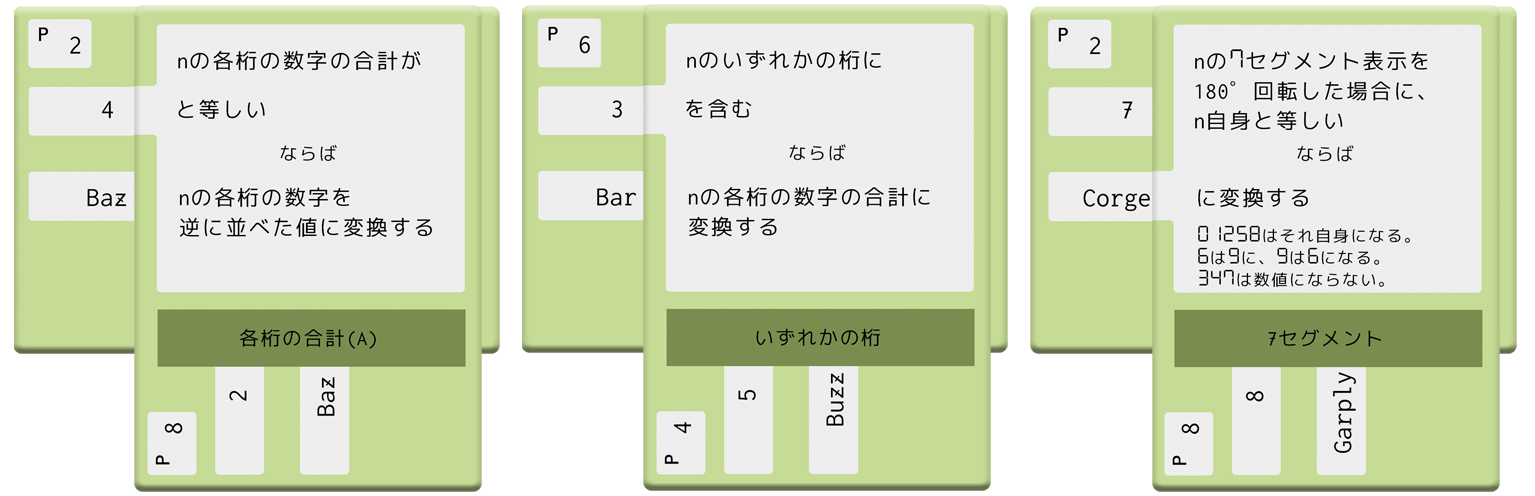
\includegraphics[height=4cm]{image/215_replay_2_5.png}
\end{center}

今はこのように変換ルールが並んでいます。このとき各変換ルールは「横向きで下に重ねられた指標カード」と「縦向きで上に重ねられた仕様カード」の2枚組で表されているわけですが、これらを組み合わせはそのまま入れ替えてしまうわけです。

その結果、あらたに有効になる変換ルールがこちらになります。

\begin{center}
  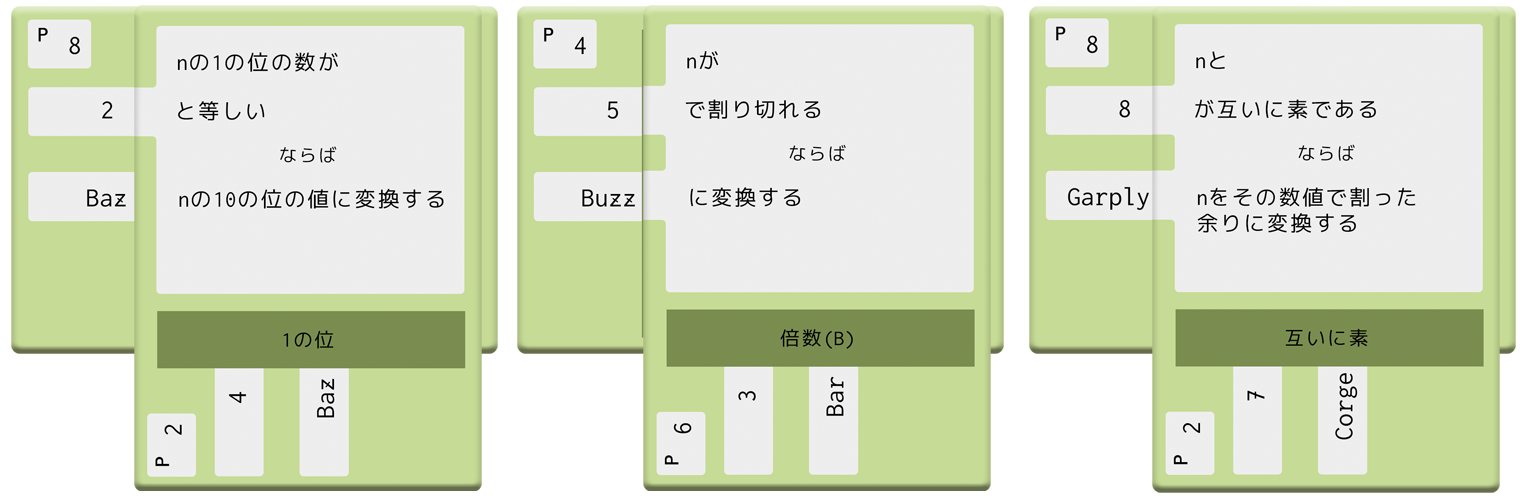
\includegraphics[height=4cm]{image/216_replay_2_6.png}
\end{center}

\begin{itembox}[l]{ローテーション後の変換ルール}
{\sf 1の位}

\hspace{1em}Pの数値: 8

\hspace{1em}nの1の位の数が2と等しいならば、nの10の位の値に変換する

{\sf 倍数(B)}

\hspace{1em}Pの数値: 4

\hspace{1em}nが5で割り切れるならば、Buzzに変換する

{\sf 互いに素}

\hspace{1em}Pの数値: 8

\hspace{1em}nと8が互いに素であるならば、nをその数値(8)で割った余りに変換する
\end{itembox}

圧倒的総入れ替え……! まぁ仕様カードが全部違うカードになるので当然なんですが。

ここまで来ると、修正というよりは1から書き直すようなものですね。「1の位」のルールで\verb+Digits+は使えそうですが、7セグメントはお役御免です。短い命だった……

まぁ、ざくっと実装していきましょう。まずは「1の位」ルールのために\verb+Digits+に新たなメソッドを生やしつつ、不要なメソッドを消します。

\begin{lstlisting}
class Digits
  def initialize(n)
    @digits = [n / 100, n / 10 % 10, n % 10]
  end

  def ones_place
    @digits[-1]
  end

  def tens_place
    @digits[-2]
  end
end
\end{lstlisting}

1の位は最下位桁、つまり配列の一番最後なので\verb+@digits[-1]+で簡単に取り出すことができますね。10の位も同様です。

これで「1の位」ルールは簡単に実装できます。

\begin{lstlisting}
class Converter
  # ...
  def ones_place_rule
    @digits.tens_place if @digits.ones_place == 2
  end
\end{lstlisting}

次、「倍数(B)」のルール。これは最初のゲームと同じく剰余を使えば簡単ですが、今回はちょっと別の方法で実装してみましょう。

5の倍数は5, 10, 15, 20, ...と、1の位の数字が必ず0か5になるという特徴があります。そして先ほど\verb+Digits+に1の位の数字を取るメソッドが生えたので、以下のような実装でも5の倍数を判定することができます。

\begin{lstlisting}
class Converter
  # ...
  def multiple_of_5_rule
    'Buzz' if [0, 5].member?(@digits.ones_place)
  end
\end{lstlisting}

最後に「互いに素」のルール。これもぱっと見は複雑そうですが、「8と互いに素」ということは「8と共通の約数を1以外に持たない」ということです。ここで $8 = 2 ^ 3$ と素因数分解できることを考えると、これは実は「2で割り切れない」、すなわち「奇数である」と等価な条件になっています。

というわけで、判定は奇数かどうかだけを見ることにしてしまいましょう。さらにこれも、奇数は「1の位の数字が1,3,5,7,9のいずれか」なので以下のように書くことができます。

\begin{lstlisting}
class Converter
  # ...
  def relative_primes_rule
    @n % 8 if [1, 3, 5, 7, 9].member?(@digits.ones_place)
  end
\end{lstlisting}

実装が「互いに素」というルールをあまり表現していないですが、わざわざ素因数分解するのも無駄なのでこれで良いでしょう。

さて、これで材料が揃ったので\verb+convert+メソッドを書き換えてしまいましょう。これもまた優先度に気をつけて並べます。

\begin{lstlisting}
class Converter
  # ...
  def convert
    relative_primes_rule || ones_place_rule || multiple_of_5_rule || @n
  end
\end{lstlisting}

  \subsection{5枚目: ★★★テンパズル}

最初のゲームと比べて、本当に難易度の高いカードばかり固め引きしている気がしますね…… 最後の★★★がどうなるか、なかなか恐ろしいところですが思い切って引いていきましょう。
  
\begin{center}
  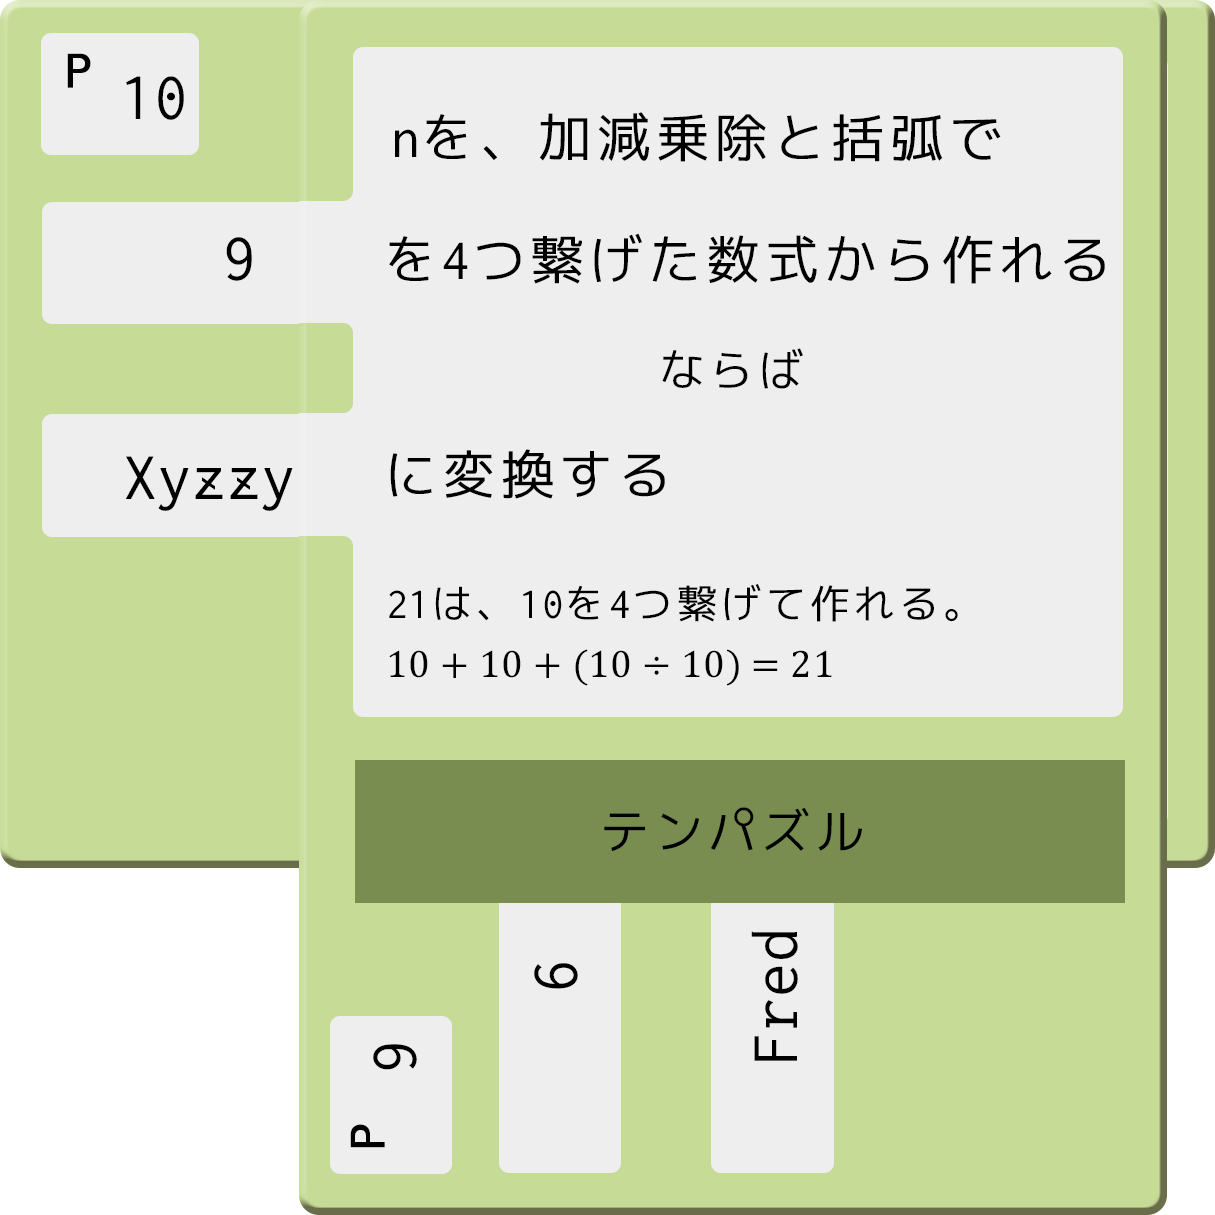
\includegraphics[height=4cm]{image/217_replay_2_7.png}
\end{center}

\begin{itembox}[l]{テンパズル}
Pの数値: 10

nを、加減乗除と括弧で9を4つ繋げた数式から作れるならば、Xyzzyに変換する

(21は、4つの10から以下のように作れる)
$10 + 10 + (10 ÷ 10) = 21$
\end{itembox}

内心、「見事にフラグを回収したな」という感じです。

テンパズルは「ナンバープレートの4つの数字を、演算子と括弧で繋いで10にできるか」というゲームです。信号待ちの暇つぶしなどで有名ですね。今回はナンバープレートのようなランダムな数字の代わりに、9を4つ使って特定の数字を作れるかを解くことになります。

さすがにこれは、少し戦略を立てないと実装できなさそうですね。

$9 □ 9 □ 9 □ 9$ という形の数式に演算子を埋める場合、演算子は $+, -, \times, \div$ の4種類しかないため、埋め方は $4^3 = 64$ 通りしかないことになります。まずはこのパターンを全て作ってみましょう。

\begin{lstlisting}
class TenPuzzle
  # 利用できる演算子
  OPERATIONS = [:+, :-, :*, :/]
  
  def all_op3
    # 演算子は必ず3つ並べるので、全ての組み合わせを作る
    # e.g. [:+, :/, :*]
    OPERATIONS.product(OPERATIONS).product(OPERATIONS)
      .map(&:flatten)
  end

  # ...
\end{lstlisting}

\verb+Array#product+ を使って、配列同士の直積を作ります。この際、2回\verb+product+を取ると最初の分が1段深くネストするため、\verb+flatten+で一次配列に整えています。

次はこれを9の間に挟み込んで式の形を作ります。ただし文字列にしてしまうとこの後の処理で扱いづらくなるので、演算子はシンボルのまま、9と演算子を並べた配列を作ることにしましょう。

\begin{lstlisting}
class TenPuzzle
  # ...

  def all_exps
    # 9を演算子の間に挟む(小数になる演算に備えてRationalにしておく)
    # e.g. [9, :+, 9, :/, 9, :*, 9]
    rat9 = Rational(9)
    exps = all_op3.map do |op3|
      [rat9, rat9, rat9, rat9].zip(op3).flatten.slice(0..-2)
    end   
  end

  # ...
\end{lstlisting}

ぱっと見ると何をしているのか分かりづらいですが、ブロックの中では \verb+[9, 9, 9, 9]+ と \verb|[:+, :/, :*]| のような配列とでzipを取っています。

この結果、\verb|[[9, :+], [9, :/], [9, :*], [9, nil]]| といった形の配列が得られます。

これを\verb+flatten+にかければだいたい求めた配列になるのですが、末尾のnilが邪魔なので最後に\verb+slice+を使って取り除いています。

なおコメントにもある通り、この後の処理で除算を行う際に割り切れない式になる場合があります。このときに\verb+Integer+だと切り捨てられてしまい本来作れない数値が答えとして得られてしまうことになるため、9は有理数型の値を使うようにしています。

さて、問題はこの式からどういった数字が作れるのかです。同じ演算子の組み合わせを使った式でも、括弧を使って評価順を変えることで得られる値が変わってきます。そこで、今回は「いずれかの演算子を選び、その前後の数で評価して新しい数式を得る」ことを繰り返すアプローチを取ってみましょう。

例えば\verb|[9, :+, 9, :/, 9, :*, 9]|という配列で考えてみると、最初に評価する演算子によって以下の3パターンに分かれます。

\begin{itemize}
\item \verb|:+|を評価: \verb|[18, :/, 9, :*, 9]|
\item \verb|:/|を評価: \verb|[9, :+, 1, :*, 9]|
\item \verb|:*|を評価: \verb|[9, :+, 9, :/, 81]|
\end{itemize}

このように評価を繰り返せば、ある数式で評価順を変えた場合に得られる値を全て集めることができます。このアプローチで組んだのが以下の\verb+solve_all+です。

\begin{lstlisting}
class TenPuzzle
  # ...

  def initialize
    @results = {}
  end
  
  def solve_all
    # 全ての順の組み合わせを試して解を記憶する
    all_exps.each { |exp| solve_exp(exp, exp, []) }
  end

  def solve_exp(exp, original_exp, orders)
    len = exp.length
    # 要素が1つしかなく、それが整数であれば、その要素を解に追加
    if len < 2
      if exp[0].denominator == 1
        @results[exp[0].to_i] ||= [original_exp.join, orders]
      end
      return
    end

    # 演算子(奇数番目要素)のそれぞれについて、評価した結果を再帰
    (1..(len / 2)).each do |i|
      op_index = i * 2 - 1
      # 対象演算子と両隣の数値で演算した結果
      center = exp[op_index - 1]
        .send(exp[op_index], exp[op_index + 1])
      # 対象演算子より2つ以上左側の部分配列
      left_exp = exp[0...(op_index - 1)]
      # 対象演算子より2つ以上右側の部分配列
      right_exp = exp[(op_index + 2)...len]
      new_exp = [left_exp, center, right_exp].flatten
      solve_exp(new_exp, original_exp, orders + [i])
    rescue ZeroDivisionError
      # 0除算が発生する組み合わせは無視する
      next
    end
  end
end
\end{lstlisting}

だいぶ複雑に見えますが、やっている処理は先ほど書いたとおり「1つの演算子に着目し、それを両隣の数字と演算して新しい式を作る」ということだけです。テクニカルな部分があるとすれば左右の部分配列の取り方で、余りの部分がない場合に空配列になるよう、終端を含まないRange(ドット3つの表記)を利用しています。

また得られた解が正しいかを確認しやすいよう、元の式を表す配列と、演算子の評価順とを組にして保存しています。

だいぶ大掛かりになりましたが、これを使って\verb+Converter+にルールを追加したらようやく終わりです。

\begin{lstlisting}
class Converter
  # ...

  def ten_puzzle_rule
    'Xyzzy' if @solver.solvable?(@n)
  end
  
  def convert
    ten_puzzle_rule || relative_primes_rule || ones_place_rule 
      || multiple_of_5_rule || @n
  end
end
\end{lstlisting}

試しに、「どの式と評価順でその数を作ったか」のデバッグ出力を有効にし、1から10までの数字で出力した結果を以下に示します。

\begin{lstlisting}
["9+9-9/9", [1, 1, 1]] => Xyzzy
["9/9+9/9", [1, 2, 1]] => Xyzzy
["9+9+9/9", [1, 1, 1]] => Xyzzy
4
5
6
["9-9+9/9", [2, 2, 1]] => Xyzzy
["9*9-9/9", [1, 1, 1]] => Xyzzy
["9+9-9*9", [2, 2, 1]] => Xyzzy
["9+9*9/9", [2, 1, 1]] => Xyzzy
\end{lstlisting}

最初のものであれば $((9 + 9) - 9) \div 9$ で確かに1になりますし、2つめは $(9 \div 9) + (9 \div 9)$ で2になっていますね。なお、評価順は「その時点で前から数えて何番目の演算子を評価したか」なので、配列の2番目に2と入っている場合、元の数式では3番目にある演算子が評価されたことを意味します。

これでようやくテンパズルも含めた実装が終わりました。完全なソースコードは掲載には長すぎるので省略します。

  \section{感想}
  
  カードの仕込みなどはせず実際に2ゲームを遊んでみましたが、カードの組み合わせによってかなり難易度に差が出るということがよくわかります。カードの仕組みやバリエーションを持たせる都合上、難易度に多少の差があることはわかっていましたが、初回のゲームに簡単めなカード、二回目のゲームに難しいカードが見事に偏った感があります……
  
  とはいえ、いずれのゲームも組み合わせによって「こんな書き方もできるな」という気づきがあり、なかなか楽しんでプログラミングをすることができました。

  今回はソロプレイでしたが、多人数でプレイする際は「こんなの余裕でしょ、30秒で書けるわ」「これは難しすぎるのでは」「この仕様が全部入れ替わるからチクショウ!」などとリアクションを取ってわいわい話しながらコードを書いてもらうと楽しいんじゃないかと思います。
\end{document}
